\section{Introduction}\label{sec:intro}
The behavior of a programming language is fundamentally shaped by its semantics. 
It is essential to have a clear and well-defined semantics of a programming language. 
A precise and unambiguous definition of language semantics is the foundation upon which all subsequent development and analysis of the language rely. 
Without it, the language’s behavior becomes unpredictable and unmanageable.

Two primary approaches are commonly used to define language semantics:
\begin{itemize}
  \item 
    \textbf{Declarative semantics} focuses on specifying the language’s behavior through formal, mathematical rules. 
    It rigorously defines a high-level, abstract model of the language semantics, without delving into implementation details. 
    Declarative semantics is especially valuable in theoretical contexts, such as academic research and formal verification. 
    It facilitates reasoning about language properties, like type soundness.
    \inred{(a more detailed example of the use cases of declarative style semantics)}
  \item 
    \textbf{Algorithmic semantics} utilizes detailed, stepwise instructions, typically presented in pseudocode, to define the language's behavior. 
    This approach offers a concrete, implementation-oriented view of how the language should be executed. 
    Such a style aids in human comprehension, as it aligns well with the sequential computational model in a developer's mind. 
    One example of algorithmic style semantics can be found in ECMAScript, which describes the semantics of JavaScript with abstract algorithms in well-structured English sentences.
\end{itemize}

\begin{figure}[t]
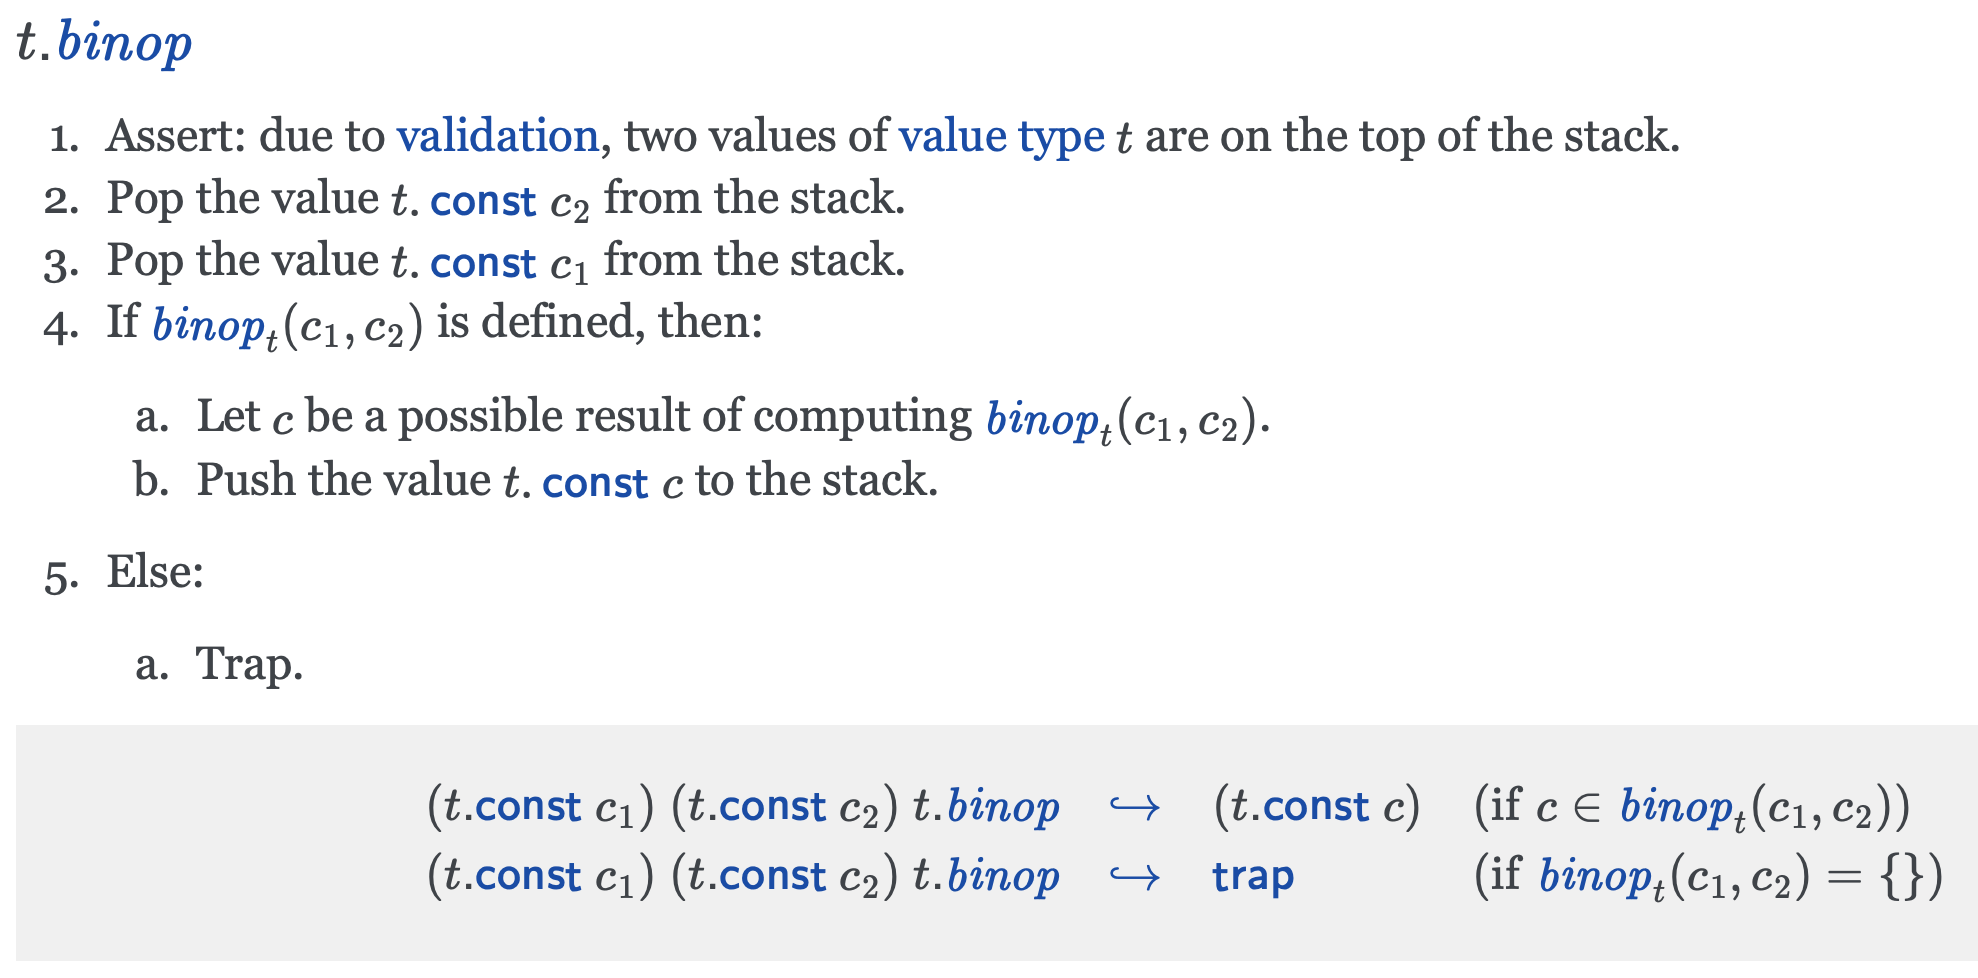
\includegraphics[width=.7\textwidth]{../img/spec.png}
\caption{The binary operator semantics in the specification}
\label{fig:spec}
\end{figure}

WebAssembly, commonly referred to as Wasm, leverages both declarative and algorithmic styles of semantic definition. 
For example, Figure~\ref{fig:spec} is the execution semantics of the Wasm $t.\mbox{\emph{binop}}$ binary operator instruction from the official specification. 
Figure~\ref{fig:spec}(a) presents the \textit{prose pseudocode} description of the $t.\mbox{\emph{binop}}$ binary operator instruction. 
The execution of the instruction is broken down into five sequential steps. 
Below, Figure~\ref{fig:spec}(b) specifies the operational semantics in rewrite rules, operating on an implicit stack of values and instructions.  
\inred{(elaborate on the "implicit stack", if necessary)}
Although in different styles, the prose and rewrite rules must be equivalent in terms of the behavior being specified.

The two styles of semantics cater to the dual needs of \textit{spec writers} and \textit{readers}. 
The prose pseudocode aids spec readers in comprehending the language implementation, providing explicit guidance. 
The sequential steps add a computational sense to the execution semantics. 
On the other hand, the rewrite rules serve the needs of spec writers, focusing on clarity and correctness of the language semantics. 
The system of rewrite rules can also be proved of type safety with assistance of interactive theorem provers, ensuring Wasm's safety from construction.

Harmonizing the dual needs of spec writers and readers, as reflected in the two semantics representations, becomes crucial when maintaining Wasm.
Wasm is a versatile technology, initially introduced as an efficient compilation target and execution model in Web platforms. 
However, flexibility of the Web environment exposes Wasm to the risk of implementation discrepancies.  
Various browsers implement Wasm within vendor-specific architectures with multi-tier interpretation or just-in-time compilation. 
In the absence of a clear prose model of Wasm semantics, aligning the behavior of the implementations and the rewrite rules will be non-trivial. 
This disparity is likely to lead to divergence in Wasm implementations, which is unfavorable since Wasm programs may fail to be protable across various platforms. 
Conversely, the absence of the formal rewrite model can also put theoretical studies of Wasm in divergence, as Wasm can be modeled in various operational semantics.  

In effort to keep the two complementary needs in sync within the standard, the W3C Wasm Community Group has established a meticulous standardization process. 
Four key artifacts are required for a feature to be standardized in Wasm:
\begin{itemize}
  \item a \textit{formal specification} for the feature in declarative-style rewrite rules, written in LaTeX;
  \item a \textit{prose pseudocode} presenting an algorithmic-style semantics, written in reStructuredText markup;
  \item an extended \textit{reference interpreter} with the implementation of the feature, written in OCaml; and
  \item a \textit{unit test suite} for the feature, written in the Wasm text format.
\end{itemize}

In contrast to the sophisticated standardization process, every piece of the Wasm specification thus far has been \textit{manually}, and thereby painstakingly written. 
This poor authorship support introduces several challenges in preparing and maintaining the Wasm specification:
\begin{itemize}
  \item 
    \textbf{Properly typesetting the specification is a tedious and labor-intensive task.} 
    \inred{(quotes from spec authors)}
  \item
    \textbf{Raw source of the specification text lacks visual clarity.} 
    Code reviews on feature proposals become a nightmare when the gist of the language is occluded by LaTeX and reStructuredText constructs. 
  \item 
    \textbf{Manual processes are susceptible to human error, potentially leading to inconsistencies or inaccuracies in the specification.} 
    The specification text surely contains errors, since human eyes are the only barrier to them. 
    Moreover, the dual semantics representation opens the door to a wide range of errors, from mainly three sources: rewrite rule itself, prose itself, and the congruence of the two styles.
    Errors in rewrite rules span from simple typos to misuse of mathematical symbols. 
    The prose may not be consistent in the English expressions, and can even contain some free variables. 
    \inred{(error example in the congruence, if exists)}
  \item 
    \textbf{Maintaining a manual specification becomes increasingly challenging as Wasm evolves.} 
    Wasm is a growing language that continually accepts proposals to add features. 
    After its initial release in 2017 as version 1.0, several proposals, including SIMD, were merged into the official specification in 2022, bumping up to version 2.0. 
    Currently, proposals including Garbage Collected Types, Threads, and Exception Handling are being developed to comprise Wasm 3.0. 
    Manual efforts are not scalable in the face of future proposals.
\end{itemize}

These challenges call for the need to automate, or \textit{mechanize} the standardization process. 
To mechanize a language definition is to define a structured representation for it, thereby allowing its automatic manipulation. 
When coupled with an execution engine, mechanized language semantics can even be executed. 
The choice of mechanization method critically depends on the aforementioned style of semantics utilized in the language specification.

For declarative-style semantics, general-purpose language frameworks such as PLT-Redex and the K framework have been developed. 
These frameworks excel in model checking and verification. 
PLT-Redex specializes in actuating the rewrite rules with evaluation contexts. 
Model checking can then be applied to the rewrite system, to debug the language semantics. 
The K framework is also a rewrite-based executable semantic framework. 
From language specification written in their language K, it generates language tools including interpreters, model checkers, and verifiers.
The K framework has been applied to specify and debug the core semantics of real-world programming languages such as C, Java, Python, and JavaScript.

Algorithmic-style semantics, as exemplified in ECMAScript, find mechanization in the ESMeta toolchain. 
ESMeta parses the structured English prose and translates them into an internal representation, $IR_{ES}$. 
$IR_{ES}$ has its own semantics, and thus can be executed with an interpreter implementation. 
Executing the JavaScript semantics written in $IR_{ES}$ allows an indirect execution of JavaScript programs. 
Utilizing the executable semantics, ESMeta derives a type checker for the specification, test suite synthesizers, and a static analyzer of JavaScript. 
Notably, ESMeta has been gracefully integrated into the continuous integration (CI) system of ECMAScript as of 2022.

\begin{figure}[t]
\footnotesize
\begin{verbatim}
rule Step_pure/binop-val:
  (CONST nt c_1) (CONST nt c_2) (BINOP nt binop) ~> (CONST nt c)
  -- if $binop(binop, nt, c_1, c_2) = c

rule Step_pure/binop-trap:
  (CONST nt c_1) (CONST nt c_2) (BINOP nt binop) ~> TRAP
  -- if $binop(binop, nt, c_1, c_2) = epsilon
\end{verbatim}
\caption{The binary operator semantics in SpecTec DSL}
\label{fig:dsl}
\end{figure}

Acknowledging the absence of a mechanization framework that utilizes both declarative and algorithmic styles, we introduce \textbf{SpecTec}, a tailored language framework that \textit{mechanizes} the Wasm standardization process. 
SpecTec defines a \emph{Domain-Specific Language (DSL)} as Wasm's single source of truth, succinctly describing the syntax, type system, and execution semantics of Wasm. 
In contrast to the official specification, the DSL deliberately and exclusively chooses a declarative style to document the execution semantics. 
Figure~\ref{fig:dsl} illustrates the semantics of $t.\mbox{\emph{binop}}$ instruction in the DSL. 
The semantics in the DSL is in close resemblance with the official formal notations in Figure~\ref{fig:spec}(b). 
Once the Wasm specification is articulated using the DSL, numerous other representations of the language can be automatically generated. 
SpecTec envisions to derive language backends dwelling in the two semantic domains:
\begin{itemize}
  \item
    \textit{Declarative backends}, including LaTeX for the formal notations and mechanized definitions in interactive theorem provers.
  \item
    \textit{Algorithmic backends}, with reStructuredText for the prose pseudocode and a Wasm interpreter.
\end{itemize}
The vision of SpecTec offers a substantial amount of automation to the current, handcrafted Wasm standard. 

SpecTec's DSL offers a clear and assisted method of defining and reasoning in the declarative backends.
The LaTeX backend augments the declarative style DSL with LaTeX constructs to produce a LaTeX document of the Wasm specification. 
Moreover, DSL is typed to prevent simple typos and arity mismatches when using parametric expressions in the rewrite rules. 
This automation streamlines authoring endeavors and guards against errors in the specification document.  
The declarative language definition can also be translated into mechanized definitions in interactive theorem provers, Coq, Isabelle, Lean, and Agda. 
Language designers can save their time and effort in manually specifying the language in various theorem provers at each specification updates. 

SpecTec's algorithmic backends are laid out by \emph{AL (Algorithmic Language)}, our meta-level language designed to describe the Wasm sementics. 
AL is carefully designed after the existing prose of Wasm specification. 
By design, converting AL programs to English prose with reStructuredText markup becomes a straightforward task. 
Furthermore, as in the approach of ESMeta, we have defined the semantics of AL with an interpreter implementation. 
This enables an indirect execution of Wasm programs. 
Our generated AL, along with the AL interpreter boasts a 100\% pass rate against the current official test suite, except for the SIMD features.

A significant challenge arises in transforming the declarative-style formal rules in DSL to algorithmic-style prose pseudocode in AL.
Bridging the gap between the two styles is a non-trivial task due to several reasons. 
To name a few, while there can be multiple rewrite rules for a single Wasm instruction, each expressing certain premises, there should be only one prose pseudocode for each instruction. 
Additionally, the equals operator '$=$' in the mathematical rules becomes ambiguous in computational sense, of whether it means an assignment or a condition check.  
Despite the differences in style, we have devised a mechnism to derive the algorithmic AL from the declarative DSL. 
We identify that the transformation is a NP-hard problem, and propose a novel solution.

SpecTec is available open source, currently documenting all of Wasm 2.0 except for the SIMD feature. 
\inred{(some coverage of the 2.0 specification?)}
SpecTec claims to be forward-compatible, even for upcoming Wasm 3.0. 
Surprisingly, specifying Wasm 3.0 in SpecTec only required minor tweaks to the tool. 
In the process, we reported several errors in the Garbage Collected Types proposal and got approval from the proposal champions. 

Our contribution is \textbf{SpecTec}, a comprehensive toolchain for the Wasm specification:
\begin{itemize}
  \item 
    \textbf{SpecTec allows spec writers to concisely specify the syntax and semanatics of Wasm.} 
    \inred{(LoC comparison)}
  \item 
    \textbf{SpecTec automatically generates backends constituting the requirement of the Wasm standardization process.}
    \inred{(self-explanatory?)}
  \item 
    \textbf{SpecTec is the first language semantics framework to embrace both declarative and algorithmic styles of semantics.}
    \inred{(also self-explanatory)}
  \item 
    \textbf{SpecTec is a barrier against meta-level errors in the specification.}
    \inred{(type checks in El/IL and errors caught by executing the AL)}
  \item 
    \textbf{SpecTec is a forward-compatible toolchain that can adapt to the evolving Wasm semantics.} 
    \inred{(case study of 3.0 proposal, maybe Exception Handling?)}
\end{itemize}
